%!TEX root = ../main.tex
\section{Aim of the Experiment}

In the experiment, the magnetization curves of different magnetic materials are determined. The $\textbf{magneto-optical Kerr effect (MOKE)} $ is used. In this effect, the linearly polarized light reflected from the magnetic material undergoes a rotation of the plane of polarization. The angle of rotation $\Phi_K$ can therefore be used to draw conclusions about the magnetization. For this purpose, different layer systems consisting of ferro-, anti-ferro- and ferrimagnetic components are used.


\section{Polarisation}

The polarization of an electromagnetic wave describes the direction of oscillation of the component of the electric field in relation to the direction of propagation. A distinction is made between linear, circular and elliptical polarization. By superposition of a right circular polarized $\Vec{E}^-$- and a left circular polarized $\Vec{E}^+$-wave a linear polarized wave can be represented. For a circularly polarized wave, the magnitude of the electric field $|\Vec{E}|$ is constant, but its direction rotates at a constant rate in the polarization plane. 
\begin{equation}
    \Vec{E}_0 = \Vec{E}^+ + \Vec{E}^- \qquad \text{with:} \qquad E^{\pm}=\frac{E_0}{2} 
    \left (
    \begin{array}{c}
         1 \\
         \pm i\\
         0\\
    \end{array}
    \right)
    \label{eq:pol}
\end{equation}

\section{Magnetic field in matter}
Due to atomic magnetic dipole moments, materials possess magnetic properties. The sum of all atomic magnetic moments $\Vec{m}_i$ divided by the volume gives the magnetization:
\begin{equation}
    \Vec{M} = \frac{\Vec{m}}{V}.
\end{equation}
Thus, the magnetic flux density can be determined to:
\begin{equation}
    \Vec{B} = \mu_0 \Vec{H} + \mu_0\Vec{M} =\mu_0\mu\Vec{H} \qquad with: \qquad \mu=1+\chi_m.
\end{equation}
Here $\chi_m$ is equal to the magnetic susceptibility.

\section{Magneto-optical Kerr effect}

The \textbf{MOKE} changes the direction of polarization and intensity of the light beam reflected from a magnetic layer system. The effect results from the side diagonal elements of the permittivity tensor $\epsilon$. This results in an anisotropic permitivity and finally in a direction dependent phase velocity in the medium with:
\begin{equation}
    v_p = \frac{c}{\sqrt{\epsilon_r\mu_r}}.
\end{equation}
Different geometries can now be distinguished, the magnitude of the effect typically decreases by one order in each case.  \begin{figure}
    \centering
    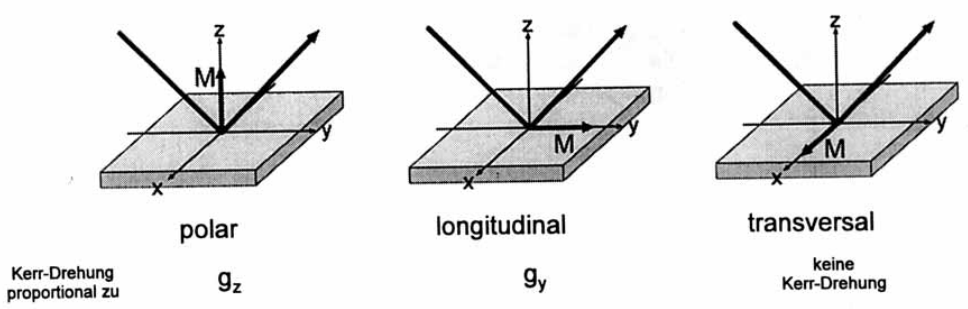
\includegraphics[height=4.0cm]{./fig/kerr-pol.png}
    \caption{Ilustration of MOKE with different geometries}
    \label{fig:kerr1}
\end{figure}
The \textbf{polar} MOKE occurs when magnetization is perpendicular to the surface, this has the greatest influence. Furthermore, the \textbf{longitudinal} MOKE occurs when the magnetization is oriented parallel to the surface and to the plane of incidence of light. Lastly, the \textbf{transversal} MOKE occurs when the magnetization is parallel to the surface but perpendicular to the optical plane. 

We consider for simplicity a perpendicular incident beam, the refractive index of a circularly polarized wave can thus be determined by:
\begin{equation}
    \Vec{n}^{\pm} \approx \Vec{n}_0\,\left (1\pm\frac{\hat{n}_0\cdot\Vec{g}}{2} \right).
\end{equation}
Where $\hat{n}_0$ is the unit vector parallel to the propagation direction ($\hat{k}$) and $\Vec{g}$ is the gyration vector with $Q = |\Vec{g}|$ being the Voigt constant. It follows that with $\Vec{g}\parallel \hat{n}_0$ for the reflection coefficient:
\begin{equation}
    r^{\pm} = \frac{n_0\cdot(1\pm0.5\cdot Q))-1}{n_0\cdot(1\pm0.5\cdot Q))+1}
\end{equation}
Choosing an incident EM wave parallel to the x-axis and the magnetization in the z-direction, i.e., the surface in the x-y plane, it follows:
\begin{align}
    \Vec{E}i= \frac{E_0}{2}
    \left [
    \left (
    \begin{array}{c}
          1\\
          i\\
          0\\
    \end{array}
    \right )
    +
    \left (
    \begin{array}{c}
          1\\
         -i\\
          0\\
    \end{array}
    \right )
    \right ] 
\end{align}

\begin{equation}
    \Vec{E}^r=r^+\Vec{E}^{i,+}+r^-\Vec{E}^{i,-}=\left ( E_0 \frac{n_0-1}{n_0+1}\cdot \Vec{e}_x + \frac{n_0\cdot Q}{(n_0+1)^2} \cdot i\Vec{e}_y \right )
\end{equation}
Here terms proportional to $Q^2$ were neglected. One recognizes a y-component of the reflected electric field as a result from the Kerr effect. The complex Kerr angle is then given by:
\begin{equation}
    \Phi_K = \frac{E^r_y}{E^r_x} = in_0Q\frac{1}{n_0^2-1}
    \label{eq:phi-kerr}
\end{equation}
Considering a purely real $n_0$, there is no rotation of the plane of polarization. The Kerr angle corresponds to the phase shift of the two waves. The reflected wave is therefore elliptically polarized. For a complex $n_0$ one obtains a real Kerr angle and thus an additional change of the plane of polarization.



\section{Magnetic anisotropy}
Die magnetische Anisotropie beschreibt eine Vorzugsrichtung bei der Magnetisierung eines Materials. Sie wird beschrieben durch die magnetische Anisotropieenergie. Die Arbeit, die benötigt wird, um die Magnetisierung $\Vec{M}$ in einem geschlossenen System ohne Teilchenaustausch aus der leichten Richtung herauszudrehen. Die leichte Richtung entspricht dabei der energetisch bevorzugten Richtung von spontaner magnetisierung. Als mikroskopische Ursache der magnetischen Anisotropie dient die Dipol-Dipol-Wechelwirkung und die Spin-Bahn-Kopplung. \\
Durch eine thermodynamische Betrachtung kann man die Gibbs'sche freie Energie bestimmen durch:
\begin{equation}
    F = -J_SH\cos(\Theta-\Theta_H) + K_{eff} \sin^2(\Theta) \qquad \text{with:} \qquad J_S = \mu_0M_S
\end{equation}
Hierbei sind:
\begin{itemize}
    \item $M_S$: magnetische Polarisation
    \item $M_S$: Sättigungsmagnetisierung
    \item $H$: Betrag des angelegten Magnetfelds
    \item $\Theta_H$: Winkel zwischen der Flächennormalen um dem Magnetfeld
    \item $\Theta$: Winkel zwischen der Flächennormalen und der Magnetisierung
    \item $K_{eff}$: die effektive Anisotropiekonstante
\end{itemize}
Die Anisotropiekonstante ist dabei gegeben durch:
\begin{equation}
    K_{eff} = -\frac{J_s^2}{2\mu_0}+K_1+\frac{2k_s}{d},
\end{equation}
die Terme sind beschreiben dabei die Formanisotropie, magnetokrisstalline Anisotropie hexagonaler Symmetrie und die Grenzflächenanisotropie. $K_{eff}$ entspricht dabei der Fläche unter der Magnetisierungskurve. \\
Die freie Energie ist ein thermodynamischen Potential und strebt im thermodynamischen Gleichgewicht ein Minimum an. Beim polaren MOKE gilt $\Theta_H = 0$, dadurch kann die Anisotropiekonstante beim Erreichen der Sättigung des Materials durch die Gleichgewichtsbedingung bestimmt werden.
\begin{align}
    \frac{dF}{d\Theta} = 0 \\
    \Rightarrow K_{eff} = -\frac{1}{2}\mu_0M_SH = -\frac{1}{2}J_S
\end{align}
Durch die Messung der Hysteresekurve muss noch die Koerzitivfeldstärke $H_C$ von der Sättigungsfeldstärke $H_S$ abgezogen werden. Außerdem ist der Kerrwinkel $\Phi_S$ im Sättigungsbereich proportional zur Sättigungsmagnetisierung. 
\begin{equation}
    J_S \propto \Phi_S
\end{equation}
Damit können wir die effektive Anisotropiekonstante berechnen zu:
\begin{equation}
    K_{eff} \propto -\frac{1}{2}\Phi_S(H_S-H_C)
\end{equation}



Magnetic anisotropy describes a preferred direction in the magnetization of a material.  It is described by the magnetic anisotropy energy, the work required to rotate the magnetization $\Vec{M}$ out of the easy direction in a closed system without particle exchange. The easy direction corresponds to the energetically preferred direction of spontaneous magnetization. The microscopic cause of the magnetic anisotropy is the dipole-dipole interaction and the spin-orbit coupling. \\
By a thermodynamic consideration, one can determine the Gibbs free energy by:
\begin{equation}
    F = -J_SH\cos(\Theta-\Theta_H) + K_{eff} \sin^2(\Theta) \qquad \text{with:} \qquad J_S = \mu_0M_S
\end{equation}
Where:
\begin{itemize}
    \item $M_S$: magnetic polarization
    \item $M_S$: Saturation magnetization
    \item $H$: magnitude of the applied magnetic field
    \item $\Theta_H$: Angle between the surface normal and the magnetic field
    \item $\Theta$: Angle between the surface normal and the magnetization
    \item $K_{eff}$: the effective anisotropy constant
\end{itemize}
Here, the anisotropy constant is given by:
\begin{equation}
    K_{eff} = -\frac{J_s^2}{2\mu_0}+K_1+\frac{2k_s}{d},
\end{equation}
the terms are describing the shape anisotropy, magnetocrisstalline anisotropy of hexagonal symmetry and the interface anisotropy. $K_{eff}$ corresponds to the area under the magnetization curve. \\
The free energy is a thermodynamic potential and tends to a minimum at thermodynamic equilibrium. In polar MOKE, $\Theta_H = 0$ holds, thus the anisotropy constant can be determined by the equilibrium condition when the material reaches saturation.
\begin{align}
    \frac{dF}{d\Theta} = 0 \\
    \Rightarrow K_{eff} = -\frac{1}{2}\mu_0M_SH = -\frac{1}{2}J_S
\end{align}
By measuring the hysteresis curve, the coercivity $H_C$ must still be subtracted from the saturation field strength $H_S$. In addition, the kerr angle $\Phi_S$ in the saturation region is proportional to the saturation magnetization. 
\begin{equation}
    J_S \propto \Phi_S
\end{equation}
Thus we can calculate the effective anisotropy constant to:
\begin{equation}
    K_{eff} \propto -\frac{1}{2}\Phi_S(H_S-H_C)
\end{equation}


\section{Relevant types of magnetism}
\subsection{Ferromagnetism}


\subsection{Anti ferromagnetism}



\subsection{Ferrimagnetism}